%!TeX root=../sensetop.tex
\chapter[Chapter \thechapter]{}
\lettrine[lraise=0.3]{T}{he} Palmers returned to Cleveland the next day, and the two families at Barton were again left to entertain each other. But this did not last long; Elinor had hardly got their last visitors out of her head, had hardly done wondering at Charlotte's being so happy without a cause, at Mr Palmer's acting so simply, with good abilities, and at the strange unsuitableness which often existed between husband and wife, before Sir John's and Mrs Jennings's active zeal in the cause of society, procured her some other new acquaintance to see and observe.

In a morning's excursion to Exeter, they had met with two young ladies, whom Mrs Jennings had the satisfaction of discovering to be her relations, and this was enough for Sir John to invite them directly to the park, as soon as their present engagements at Exeter were over. Their engagements at Exeter instantly gave way before such an invitation, and Lady Middleton was thrown into no little alarm on the return of Sir John, by hearing that she was very soon to receive a visit from two girls whom she had never seen in her life, and of whose elegance,—whose tolerable gentility even, she could have no proof; for the assurances of her husband and mother on that subject went for nothing at all. Their being her relations too made it so much the worse; and Mrs Jennings's attempts at consolation were therefore unfortunately founded, when she advised her daughter not to care about their being so fashionable; because they were all cousins and must put up with one another. As it was impossible, however, now to prevent their coming, Lady Middleton resigned herself to the idea of it, with all the philosophy of a well-bred woman, contenting herself with merely giving her husband a gentle reprimand on the subject five or six times every day.

The young ladies arrived: their appearance was by no means ungenteel or unfashionable. Their dress was very smart, their manners very civil, they were delighted with the house, and in raptures with the furniture, and they happened to be so doatingly fond of children that Lady Middleton's good opinion was engaged in their favour before they had been an hour at the Park. She declared them to be very agreeable girls indeed, which for her ladyship was enthusiastic admiration. Sir John's confidence in his own judgment rose with this animated praise, and he set off directly for the cottage to tell the Miss Dashwoods of the Miss Steeles' arrival, and to assure them of their being the sweetest girls in the world. From such commendation as this, however, there was not much to be learned; Elinor well knew that the sweetest girls in the world were to be met with in every part of England, under every possible variation of form, face, temper and understanding. Sir John wanted the whole family to walk to the Park directly and look at his guests. Benevolent, philanthropic man! It was painful to him even to keep a third cousin to himself.

<Do come now,> said he—<pray come—you must come—I declare you shall come—You can't think how you will like them. Lucy is monstrous pretty, and so good humoured and agreeable! The children are all hanging about her already, as if she was an old acquaintance. And they both long to see you of all things, for they have heard at Exeter that you are the most beautiful creatures in the world; and I have told them it is all very true, and a great deal more. You will be delighted with them I am sure. They have brought the whole coach full of playthings for the children. How can you be so cross as not to come? Why they are your cousins, you know, after a fashion. \textit{You} are my cousins, and they are my wife's, so you must be related.>

But Sir John could not prevail. He could only obtain a promise of their calling at the Park within a day or two, and then left them in amazement at their indifference, to walk home and boast anew of their attractions to the Miss Steeles, as he had been already boasting of the Miss Steeles to them.

When their promised visit to the Park and consequent introduction to these young ladies took place, they found in the appearance of the eldest, who was nearly thirty, with a very plain and not a sensible face, nothing to admire; but in the other, who was not more than two or three and twenty, they acknowledged considerable beauty; her features were pretty, and she had a sharp quick eye, and a smartness of air, which though it did not give actual elegance or grace, gave distinction to her person. Their manners were particularly civil, and Elinor soon allowed them credit for some kind of sense, when she saw with what constant and judicious attention they were making themselves agreeable to Lady Middleton. With her children they were in continual raptures, extolling their beauty, courting their notice, and humouring their whims; and such of their time as could be spared from the importunate demands which this politeness made on it, was spent in admiration of whatever her ladyship was doing, if she happened to be doing any thing, or in taking patterns of some elegant new dress, in which her appearance the day before had thrown them into unceasing delight. Fortunately for those who pay their court through such foibles, a fond mother, though, in pursuit of praise for her children, the most rapacious of human beings, is likewise the most credulous; her demands are exorbitant; but she will swallow any thing; and the excessive affection and endurance of the Miss Steeles towards her offspring were viewed therefore by Lady Middleton without the smallest surprise or distrust. She saw with maternal complacency all the impertinent encroachments and mischievous tricks to which her cousins submitted. She saw their sashes untied, their hair pulled about their ears, their work-bags searched, and their knives and scissors stolen away, and felt no doubt of its being a reciprocal enjoyment. It suggested no other surprise than that Elinor and Marianne should sit so composedly by, without claiming a share in what was passing.

% \begin{figure}[tbph]
% \centering
% 
\includegraphics[width=\linewidth]{21tricks}
% \caption{Mischievous tricks}
% \end{figure}

\begin{bwbigpic}
	[1.0]
	{21tricks} 
	{Mischievous tricks} 
\end{bwbigpic}

<John is in such spirits today!> said she, on his taking Miss Steeles's pocket handkerchief, and throwing it out of window—<He is full of monkey tricks.>

And soon afterwards, on the second boy's violently pinching one of the same lady's fingers, she fondly observed, <How playful William is!>

<And here is my sweet little Annamaria,> she added, tenderly caressing a little girl of three years old, who had not made a noise for the last two minutes; <And she is always so gentle and quiet—Never was there such a quiet little thing!>

But unfortunately in bestowing these embraces, a pin in her ladyship's head dress slightly scratching the child's neck, produced from this pattern of gentleness such violent screams, as could hardly be outdone by any creature professedly noisy. The mother's consternation was excessive; but it could not surpass the alarm of the Miss Steeles, and every thing was done by all three, in so critical an emergency, which affection could suggest as likely to assuage the agonies of the little sufferer. She was seated in her mother's lap, covered with kisses, her wound bathed with lavender-water, by one of the Miss Steeles, who was on her knees to attend her, and her mouth stuffed with sugar plums by the other. With such a reward for her tears, the child was too wise to cease crying. She still screamed and sobbed lustily, kicked her two brothers for offering to touch her, and all their united soothings were ineffectual till Lady Middleton luckily remembering that in a scene of similar distress last week, some apricot marmalade had been successfully applied for a bruised temple, the same remedy was eagerly proposed for this unfortunate scratch, and a slight intermission of screams in the young lady on hearing it, gave them reason to hope that it would not be rejected. She was carried out of the room therefore in her mother's arms, in quest of this medicine, and as the two boys chose to follow, though earnestly entreated by their mother to stay behind, the four young ladies were left in a quietness which the room had not known for many hours.

<Poor little creatures!> said Miss Steele, as soon as they were gone. <It might have been a very sad accident.>

<Yet I hardly know how,> cried Marianne, <unless it had been under totally different circumstances. But this is the usual way of heightening alarm, where there is nothing to be alarmed at in reality.>

<What a sweet woman Lady Middleton is!> said Lucy Steele.

Marianne was silent; it was impossible for her to say what she did not feel, however trivial the occasion; and upon Elinor therefore the whole task of telling lies when politeness required it, always fell. She did her best when thus called on, by speaking of Lady Middleton with more warmth than she felt, though with far less than Miss Lucy.

<And Sir John too,> cried the elder sister, <what a charming man he is!>

Here too, Miss Dashwood's commendation, being only simple and just, came in without any eclat. She merely observed that he was perfectly good humoured and friendly.

<And what a charming little family they have! I never saw such fine children in my life.—I declare I quite doat upon them already, and indeed I am always distractedly fond of children.>

<I should guess so,> said Elinor, with a smile, <from what I have witnessed this morning.>

<I have a notion,> said Lucy, <you think the little Middletons rather too much indulged; perhaps they may be the outside of enough; but it is so natural in Lady Middleton; and for my part, I love to see children full of life and spirits; I cannot bear them if they are tame and quiet.>

<I confess,> replied Elinor, <that while I am at Barton Park, I never think of tame and quiet children with any abhorrence.>

A short pause succeeded this speech, which was first broken by Miss Steele, who seemed very much disposed for conversation, and who now said rather abruptly, <And how do you like Devonshire, Miss Dashwood? I suppose you were very sorry to leave Sussex.>

In some surprise at the familiarity of this question, or at least of the manner in which it was spoken, Elinor replied that she was.

<Norland is a prodigious beautiful place, is not it?> added Miss Steele.

<We have heard Sir John admire it excessively,> said Lucy, who seemed to think some apology necessary for the freedom of her sister.

<I think every one \textit{must} admire it,> replied Elinor, <who ever saw the place; though it is not to be supposed that any one can estimate its beauties as we do.>

<And had you a great many smart beaux there? I suppose you have not so many in this part of the world; for my part, I think they are a vast addition always.>

<But why should you think,> said Lucy, looking ashamed of her sister, <that there are not as many genteel young men in Devonshire as Sussex?>

<Nay, my dear, I'm sure I don't pretend to say that there an't. I'm sure there's a vast many smart beaux in Exeter; but you know, how could I tell what smart beaux there might be about Norland; and I was only afraid the Miss Dashwoods might find it dull at Barton, if they had not so many as they used to have. But perhaps you young ladies may not care about the beaux, and had as lief be without them as with them. For my part, I think they are vastly agreeable, provided they dress smart and behave civil. But I can't bear to see them dirty and nasty. Now there's Mr Rose at Exeter, a prodigious smart young man, quite a beau, clerk to Mr Simpson, you know, and yet if you do but meet him of a morning, he is not fit to be seen. I suppose your brother was quite a beau, Miss Dashwood, before he married, as he was so rich?>

<Upon my word,> replied Elinor, <I cannot tell you, for I do not perfectly comprehend the meaning of the word. But this I can say, that if he ever was a beau before he married, he is one still for there is not the smallest alteration in him.>

<Oh! dear! one never thinks of married men's being beaux—they have something else to do.>

<Lord! Anne,> cried her sister, <you can talk of nothing but beaux;—you will make Miss Dashwood believe you think of nothing else.> And then to turn the discourse, she began admiring the house and the furniture.

This specimen of the Miss Steeles was enough. The vulgar freedom and folly of the eldest left her no recommendation, and as Elinor was not blinded by the beauty, or the shrewd look of the youngest, to her want of real elegance and artlessness, she left the house without any wish of knowing them better.

Not so the Miss Steeles. They came from Exeter, well provided with admiration for the use of Sir John Middleton, his family, and all his relations, and no niggardly proportion was now dealt out to his fair cousins, whom they declared to be the most beautiful, elegant, accomplished, and agreeable girls they had ever beheld, and with whom they were particularly anxious to be better acquainted. And to be better acquainted therefore, Elinor soon found was their inevitable lot, for as Sir John was entirely on the side of the Miss Steeles, their party would be too strong for opposition, and that kind of intimacy must be submitted to, which consists of sitting an hour or two together in the same room almost every day. Sir John could do no more; but he did not know that any more was required: to be together was, in his opinion, to be intimate, and while his continual schemes for their meeting were effectual, he had not a doubt of their being established friends.

To do him justice, he did every thing in his power to promote their unreserve, by making the Miss Steeles acquainted with whatever he knew or supposed of his cousins' situations in the most delicate particulars; and Elinor had not seen them more than twice, before the eldest of them wished her joy on her sister's having been so lucky as to make a conquest of a very smart beau since she came to Barton.

<'Twill be a fine thing to have her married so young to be sure,> said she, <and I hear he is quite a beau, and prodigious handsome. And I hope you may have as good luck yourself soon,—but perhaps you may have a friend in the corner already.>

Elinor could not suppose that Sir John would be more nice in proclaiming his suspicions of her regard for Edward, than he had been with respect to Marianne; indeed it was rather his favourite joke of the two, as being somewhat newer and more conjectural; and since Edward's visit, they had never dined together without his drinking to her best affections with so much significancy and so many nods and winks, as to excite general attention. The letter F—had been likewise invariably brought forward, and found productive of such countless jokes, that its character as the wittiest letter in the alphabet had been long established with Elinor.

% \begin{figure}[tbph]
% \centering
% 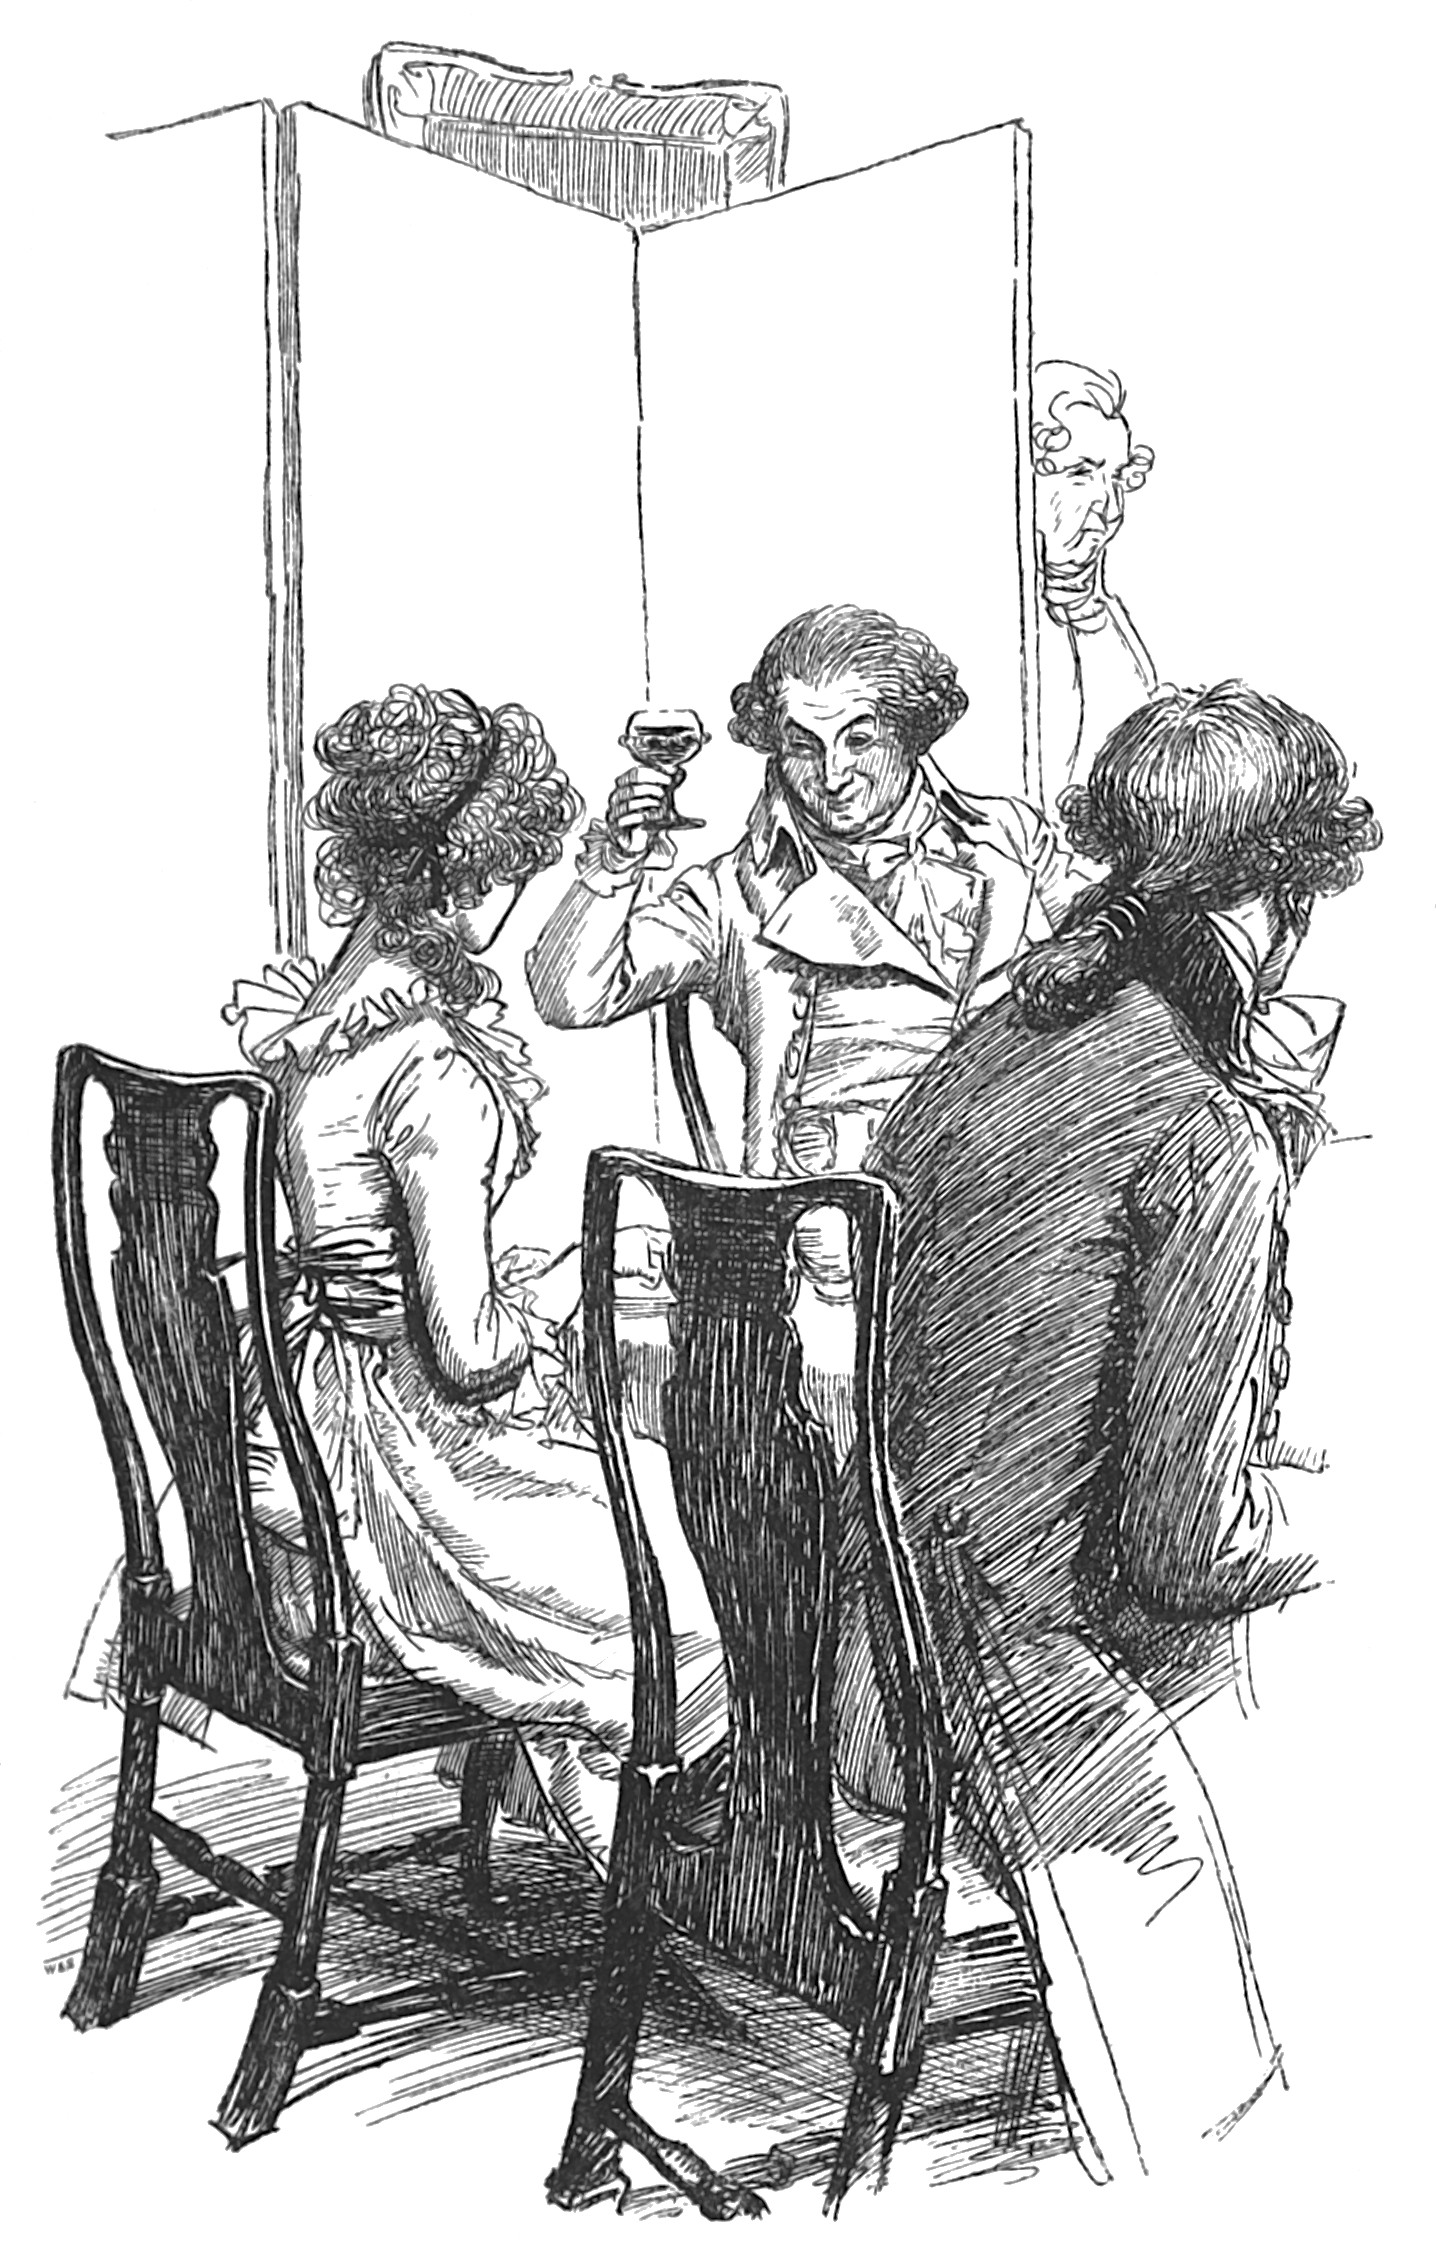
\includegraphics[width=.9\linewidth]{21drinking}
% \caption{Drinking to her best affections}
% \end{figure}



\begin{letter}
\begin{bwbigpic}
	[1.0]
	{21drinking} 
	{Drinking to her best affections} 
\end{bwbigpic}
\end{letter}
\begin{a4}
\begin{bwbigpic}
	[0.9]
	{21drinking} 
	{Drinking to her best affections} 
\end{bwbigpic}
\end{a4}

The Miss Steeles, as she expected, had now all the benefit of these jokes, and in the eldest of them they raised a curiosity to know the name of the gentleman alluded to, which, though often impertinently expressed, was perfectly of a piece with her general inquisitiveness into the concerns of their family. But Sir John did not sport long with the curiosity which he delighted to raise, for he had at least as much pleasure in telling the name, as Miss Steele had in hearing it.

<His name is Ferrars,> said he, in a very audible whisper; <but pray do not tell it, for it's a great secret.>

<Ferrars!> repeated Miss Steele; <Mr Ferrars is the happy man, is he? What! your sister-in-law's brother, Miss Dashwood? a very agreeable young man to be sure; I know him very well.>

<How can you say so, Anne?> cried Lucy, who generally made an amendment to all her sister's assertions. <Though we have seen him once or twice at my uncle's, it is rather too much to pretend to know him very well.>

Elinor heard all this with attention and surprise. <And who was this uncle? Where did he live? How came they acquainted?> She wished very much to have the subject continued, though she did not chuse to join in it herself; but nothing more of it was said, and for the first time in her life, she thought Mrs Jennings deficient either in curiosity after petty information, or in a disposition to communicate it. The manner in which Miss Steele had spoken of Edward, increased her curiosity; for it struck her as being rather ill-natured, and suggested the suspicion of that lady's knowing, or fancying herself to know something to his disadvantage.—But her curiosity was unavailing, for no farther notice was taken of Mr Ferrars's name by Miss Steele when alluded to, or even openly mentioned by Sir John.